\begin{textarea}[]
\only<1>{
\begin{algorithm}[H]
\begin{algorithmic}[1]
\FOR {$k = 1 \cdots n$}
	\FOR {$i = k+1 \cdots n$}
    	\STATE $m := A[i, k] / A[k, k]$
    	\FOR {$j = k+1 \cdots n$}
 \STATE $A[i, j]  := A[i, j] - A[k, j] * m$
    	\ENDFOR
    	\STATE $A[i, k]  := 0$
    \ENDFOR
\ENDFOR
\end{algorithmic}
\end{algorithm}
}
\only<2>{
What is the Gauss-Algorithm?
}
\end{textarea}

\begin{textarea}[]
\only<1>{
\begin{algorithm}[H]
\begin{algorithmic}[1]
\FOR {$n = size(A) \cdots 2$}
	\FOR {$i = 0 \cdots n-2$}
    	\IF {$A[i] > A[i+1]$}
 			\STATE Swap$(A[i],A[i+1])$
 		\ENDIF
    \ENDFOR
\ENDFOR
\end{algorithmic}
\end{algorithm}
}
\only<2>{
What is Bubble Sort?
}
\end{textarea}

\begin{textarea}[]
\only<1>{
\begin{algorithm}[H]
\begin{algorithmic}[1]
\WHILE {$\vert df \vert > \varepsilon $}
	\STATE $df = \text{gradientF(x)}$
	\STATE $x = x-\alpha df$
\ENDWHILE
\end{algorithmic}
\end{algorithm}
}
\only<2>{
What is Steepest Descent?
}
\end{textarea}

\begin{textarea}[]
\only<1>{
\centering
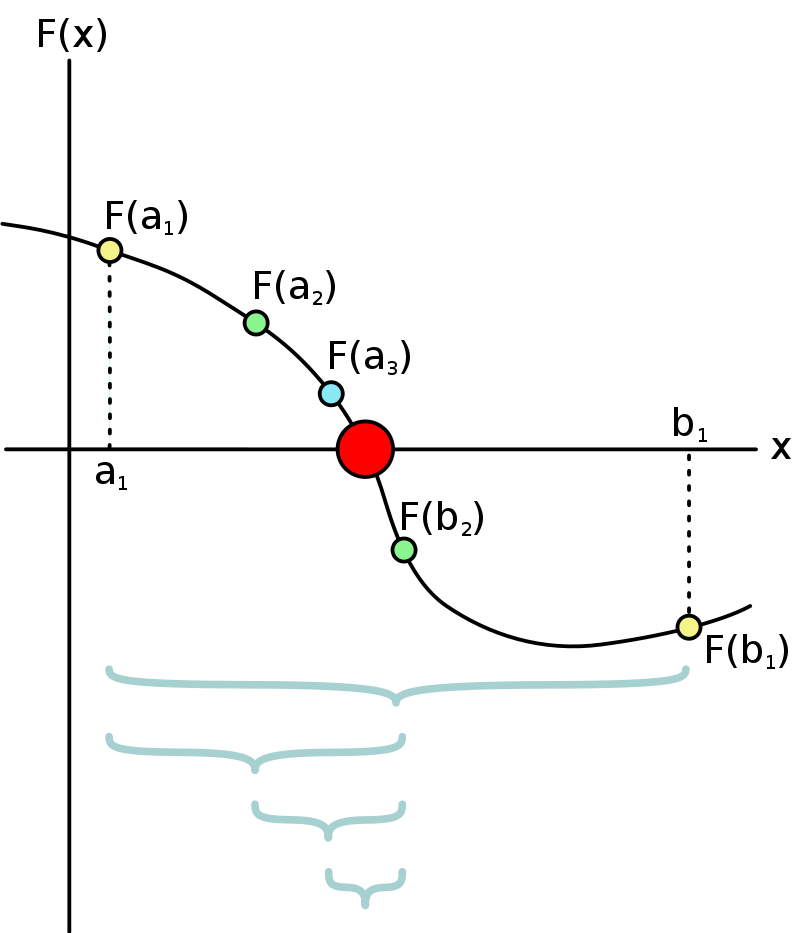
\includegraphics[height=0.5\linewidth]{categories/media/800px-Bisection_method}
}
\only<2>{
What is bisection?
}
\end{textarea}

\begin{textarea}[]
\only<1>{
\centering
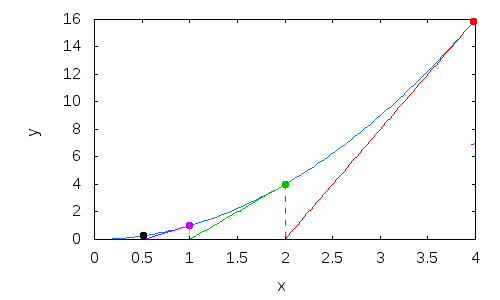
\includegraphics[height=0.5\linewidth]{categories/media/Newtons_method_x2}
}
\only<2>{
What is Newton's method?
}
\end{textarea}
